\chapter{Analysis of the ported \textsc{BaseX} Android version}
\label{cha:analysis}
The following chapter outlines how the migrated \textsc{BaseX} Android database is analyzed.
The focus at this part lies on the evaluation and the performance of the library.
First the specification of the test devices is outlined and an estimation is made to show how the performance of the various devices differ.
Therefore different benchmarks has been executed to approximate the distinctive hardware properties and their execution times.
In the next chapter is shown that the migrated database works without errors and failures on the Android mobile platform using a real devices.
For this purpose different unit test has been also migrated to test the functionality.
After evaluation the functionality the performance has been investigated.
An overview of the performance an XML benchmark set, which is especially designed to test the performance of XQuery executions, has been used.
\section{Evaluation of the test devices}
\label{sec:evaluation-of-the-test-devices}
For the measurement of the performance two devices are being used.
First, for testing the \textsc{BaseX} mobile version an Android Tablet PC Samsung Galaxy Tab 2 10.1 and for the normal \textsc{BaseX} version a Lenovo Thinkpad laptop have been used.
Their technical specifications can be seen in Table\ref{tab:test-dev-specs}.
\begin {table}[htpb] 
  \centering
\begin {tabular} {|r|r|r|r|r|r|}
  	\hline
	&CPU&RAM&filesystem&operating system\\
	\hline
	Laptop&Intel Core2 Duo CPU L7100&2 Gb&ext4&Arch Linux\\
	&1.2 GHz&&&(3.12.0)\\
	\hline
	Tablet&Dual-core Cortex-A9&1 Gb&ext4&Android\\
	&1 GHz&&&(4.0.3)\\
	\hline
\end {tabular}
\caption {The technical specifications of the two devices, used for benchmark testing.}
\label {tab:test-dev-specs}
\end {table}

Looking at this table it can be seen that the only similarity of both systems is that they are using the same filesystem, which is ext4, which is short for fourth extended filesystem.
The RAM of the laptop is the double amount of the tablet available RAM and both devices have a dual core CPU with around 1 GHz.
Even if the specifications are not so much differ on the first look, their performance varies in some factors.
Therefore a measurement of the input/output (IO) and CPU speed of booth devices has been made in Section~\ref{sec:evaluation-of-the-test-devices} to get a clearer look how the devices differ.


%\section{Evaluating the working \textsc{BaseX} Android port}
%\label{sec:evaluating-the-working-basex-android-port}
%\textbf{TODO}\\
%In this section will be shown that the created \textsc{BaseX} Android port works and fit all requirements.
%For this purpose the given JUnit tests were been migrated to Android too.
%This shows that all functions work like they work on the standard Java version.
The two devices which have been used to benchmark \textsc{BaseX} are totally different and not just in the fact that one is laptop and the other a tablet PC.
They differ in many hardware aspects, but there are two different factors, that are interesting to identify a systems speed and are used for the given purpose.
These are the CPU speed and the input/output (IO) speed, where IO speed is a headline for different operations.
Broadly speaking it can be said that the IO speed can be divided into read and write operations.\\
To measure this values the benchmark tool Bonnie++\footnote{\url{http://www.coker.com.au/Bonnie++/}} is used.
This tool executes different operations and measures how many of these operations can be executed in one second.
It tests sequential output, sequential input, random seeks, sequential create and random create.\\
The sequential output represents the write speed of the system, Bonnie++ uses three different methods to measure this value.
First it writes one character after another by using the \textit{putc()} systemcall. 
After this operation it writes whole blocks with the size of 8192 bytes by using the write() systemcall and than calling the close() systemcall.
The last test in this category is the rewrite test and differs from the write test, that the file is not closed after writing.
Therefore one block write comply with 8192 \textit{putc} calls and is way more effective and faster than writing single characters.
The next test is to measure the random seek operations per seconds, which means how often the read/write position can be changed.
It also measures the latency which represents the rotation speed of the disk, but this is obsolete because both systems have flash storage and so there is no revolution per minute to measure.
Bonny is written in C++ and is available on most Linux distributions, but to use it on Android it is necessary to build it from its sources by using the, in Chapter~\ref{sec:migration:the-android-project-structure} mentioned, Android Native Development Kit (NDK).
This provides a cross compiler which makes it possible to build C++ code for Android.
For the execution of the benchmarks the version 1.96 from Bonnie++ has been used.
The results of these test executions can be seen in table~\ref{tab:bonnie-results-out}.
%\begin {table}
%\begin {tabular} {|r|r|r|r|r|r|r|r|r|r|r|r|r|}
%	\hline
%		&\multicolumn {3} {|c|} {Sequential}&\multicolumn {2} {|c|} {Sequential}&Random&\multicolumn {3} {|c|} {Sequential}&\multicolumn {3} {|c|} {Random}\\
%		&\multicolumn {3} {|c|} {Output}&\multicolumn {2} {|c|} {Input}&Seeks&\multicolumn {3} {|c|} {Create}&\multicolumn {3} {|c|} {Create}\\
%	\hline
%		&K/sec&K/sec&K/sec&K/sec&/sec&/sec&/sec&/sec&/sec&/sec&/sec&/sec\\
%	\hline
%	Laptop&201&62180&23850&907&98239&1161&17134&137752&13032&19442&170028&11774\\
%	\hline
%	Tablet&5&20828&8756&596&23768&475.6&39&361&167&42&391&238\\
%	\hline
%	\hline
%	Factors&40.20&2.99&2.72&1.52&4.13&2.44&439.33&381.58&78.04&462.90&434.85&49.47\\
%	\hline
%\end {tabular}
%\caption {Results of the Bonnie++ benchmarks.}
%\label {tab:bonnie-results}
%\end {table}


\begin {table}[htpb] 
  \centering
\begin {tabular} {|r|r|r|r|r|r|r|}
	\hline
		&\multicolumn {3} {|c|} {Sequential}&\multicolumn {2} {|c|} {Sequential}&\multicolumn {1} {|c|}{Random}\\
		&\multicolumn {3} {|c|} {Output}&\multicolumn {2} {|c|} {Input}&\multicolumn {1} {|c|}{Seeks}\\
	\hline
		&Char&Block&Rewrite&Char&Block&\\
	\hline
	Laptop&201K&62180K&23850K&907K&98239K&1161\\
	\hline
	Tablet&5K&20828K&8756K&596K&23768K&475.6\\
	\hline
	\hline
	Factors&40.20&2.99&2.72&1.52&4.13&2.44\\
	\hline
\end {tabular}
\caption {Results of the Bonnie++ in- and output benchmarks.}
\label {tab:bonnie-results-out}
\end {table}


Bonnie++ also measures the sequential and random create of a file.
Therefore it creates, queries its status and deletes a file by using the Posix systemcalls \textit{creat()}, \textit{stat()} and \textit{unlink()}.
The results of this test can be seen in Table~\ref{tab:bonnie-results-create}
\begin {table}[htpb] 
  \centering
\begin {tabular} {|r|r|r|r|r|r|r|}
	\hline
		&\multicolumn {3} {|c|} {Sequential}&\multicolumn {3} {|c|} {Random}\\
		&\multicolumn {3} {|c|} {Create}&\multicolumn {3} {|c|} {Create}\\
	\hline
		&creat()&stat()&unlink()&creat()&stat()&unlink()\\
	\hline
	Laptop&17134&137752&13032&19442&170028&11774\\
	\hline
	Tablet&39&361&167&42&391&238\\
	\hline
	\hline
	Factors&439.33&381.58&78.04&462.90&434.85&49.47\\
	\hline
\end {tabular}
\caption {Results of the Bonnie++ sequential/random create benchmarks.}
\label {tab:bonnie-results-create}
\end {table}


%\begin {table}
%\begin {tabular} {|r|r|r|r|r|r|r|}
%	\hline
%		&\multicolumn {3} {|c|} {Sequential}&\multicolumn {2} {|c|} {Sequential}&\multicolumn {1} {|c|}{Random}\\
%		&\multicolumn {3} {|c|} {Output}&\multicolumn {2} {|c|} {Input}&\multicolumn {1} {|c|}{Seeks}\\
%	\hline
%		&Char&Block&Rewrite&Char&Block&\\
%	\hline
%	Laptop (per seconds)&201K&62180K&23850K&907K&98239&1161\\
%	\hline
%	Tablet (per seconds)&5K&20828K&8756K&596&23768K&475.6\\
%	\hline
%	\hline
%	Factors&40.20&2.99&2.72&1.52&4.13&2.44\\
%	\hline
%\end {tabular}
%\caption {Results of the Bonnie++ benchmarks.}
%\label {tab:bonnie-results}
%\end {table}


By analyzing these values it can be said that the laptop is overall faster than the tablet PC.
It is well known that IO operations are the most expensive one on Android, so the achieved result is no surprise. 
But with these values it can be said that there are factors which can tell how much faster it is in specific operations.
This factors are impossible to optimize, because they are a hardware constraint and only changing the hardware can improve them, but they are still important to identify the bottlenecks of the mobile \textsc{BaseX} version.\\
Analyzing Table~\ref{tab:bonnie-results-create} and having a look at the factors shows one value which is, compared to the other factors, extremely high.
The sequential write per character is 40 times faster on the laptop than on the tablet, considering this, it is clear to avoid writing by character instead by block.
Writing by using the block mechanism is just three times slower on the tablet.
The sequential reading of a single character is at the tablet just 1.52 times slower than the at the notebook.
Though the factor of the block reading is quite higher than the character reading factor it is sure to use the block reading because it is much faster than character reading.
But by using block reading the factor need also be considered in the \textsc{BaseX} benchmarks later in chapter~\ref{sec:analysing-the-execution-performance}.
\\
Looking at Table~\ref{tab:bonnie-results-create} it can be seen that the sequential/random creation, reading and deleting is very slow on the Android devices compared to the laptop.
Considering this it should be avoided to often create files, because this is very slow.\\
Bonnie++ gives a good overview about how fast the two system handle their IO operations and how they differ in this aspect.
But there is also another factor which affects the speed of the execution of a program.
This is the CPU speed, it is obvious that this also differs on both test devices.
To evaluate the CPU times a Java program has been written which executes four different CPU intensive operations.
First it does the naive factorial of 5000, where naive means that it just iterates till 5000 and multiplies every step to the result.
The second test is a recursive calculation of the 100th Fibonacci number.
The third sorts an ascending ordered array of 10000 items using the bubble-sort algorithm.
This is done because this is the worst case for the bubble-sort algorithm and has a complexity of $\mathcal O(n^2)$.
The last test makes a naive test if the number 666667 is prime or not, by testing to divide the number by every candidate step by step till the candidate is the square root of the number.
All these test are very CPU intensive, because they use only arithmetic operations.
The results of these test can be seen in Table~\ref{tab:cpu-results}.
\begin {table}[htpb] 
  \centering
\begin {tabular} {|l|r|r|r|r|}
	\hline
		&Factorial&Fibonacci&Bubble Sort&Prime Number\\
	\hline
	Laptop&&&&\\
	(avg. on 1000 runs)&98.19 ms&248.63 ms&180.53 ms&15.85 ms\\
	\hline
	Tablet&&&&\\
	(avg. on 1000 runs)&491.15 ms&2336.35 ms&1045.52 ms&76.41 ms\\
	\hline
	\hline
	Factors&5&9.4&5.8&4.8\\
	\hline
\end {tabular}
\caption {Results of the CPU benchmarks.}
\label {tab:cpu-results}
\end {table}


Except the Fibonacci test it can be said that the CPU of the laptop is about five times faster than the one of the laptop.
This is like the different IO parameters a factor which could not be improved and has to be considered in the \textsc{BaseX} benchmarks as well.
These evaluation is for measuring the performance of the two \textsc{BaseX} versions and how to cope with the results achieved by two different platforms on two different devices.


\section{Analyzing the execution performance}
\label{sec:analysing-the-execution-performance}
To investigate the performance of the Android version of \textsc{BaseX} the benchmark suite \textit{XMark} has been used.
\textit{XMark} creates random XML files and has a set of twenty predefined queries that can be used to measure the execution performance of an \textit{XQuery} implementation.
It offers the possibility to choose the size of the random XML files, so that the test queries can be executed on different file sizes.
Therefore it is also being used to find the maximum supported size of a \textsc{BaseX} database on Android.


\subsection{The XMark benchmark suite}
\label{subsec:the-xmark-benchmark-suite}
The XMark benchmark suite is used to identify the speed of the \textsc{BaseX} Android version.
Therefore it offers 20 different XQueries which are designed to benchmark a XQuery implementation.
The queries are separated into different categories, where every category targets a specific aspect of query execution.
The XML files that can be generated by using XMark are all containing the same elements and every file is well-formed.
The content of the generated XML files is randomly generated by using the 17000 most frequently used words~\footnote{ignoring stop words} in the plays of Shakespeare~\cite{schmidtxmark}.
The structure of the randomly generated XML files can be seen in Figure~\ref{fig:xmark-file-structure}.
\begin{figure}[htpb]
\begin{center}
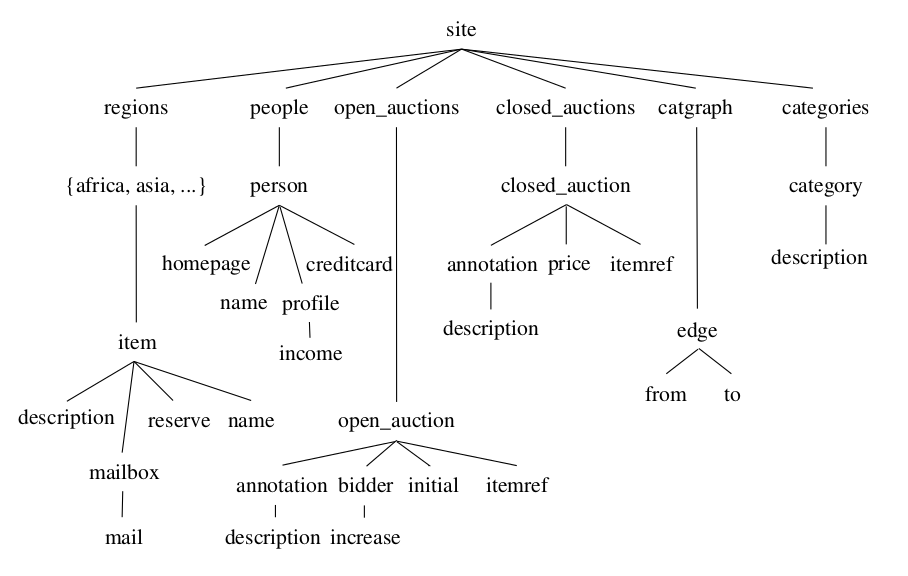
\includegraphics[scale=0.42]{images/xmark-file-elements.png} 
\caption{The structure of a generated XMark XML file. Source:\cite{schmidtxmark}}
\label{fig:xmark-file-structure}
\end{center}
\end{figure}

The size of the XML files can be chosen during the generation process of XMark.
For testing \textsc{BaseX} 15 different files were been generated.
The smallest with the size of 100 Kb followed by files with a size increasing by 100 Kb steps.
Hence, the biggest generated file has a size of 1.4 Mb.\\
The different queries can be seen in Table~\ref{tab:xmark-queries}.
\begin {table}[htpb] 
  \centering
	\begin{tabular}{r|l}
	  \hline
	  1&Return the name of the person with ID 'person0'.\\
	  \hline
	  2&Return the initial increase of all open auctions.\\
	  \hline
	  3&Return the first and current increase of all open auctions whose current\\
	  &increase is at least twice as high as the initial increase.\\
	  \hline
	  4&List the reserves of those open auctions where a certain person issued\\
	  &a bid before another person.\\
	  \hline
	  5&How many sold items cost more than 40.\\
	  \hline
	  6&How many items are listed on all continents?\\
	  \hline
	  7&How many pieces of prose are in our database?\\
	  \hline
	  8&List the names of persons and the number of items they bought.\\
	  &(Joins person, closed\_auction)\\
	  \hline
	  9&List the names of persons and the names of items they bought in Europe.\\
	  &(Joins person\_auction, item)\\
	  \hline
	  10&List all persons according to their interest; use French markup\\
	  &in the result.\\
	  \hline
	  11&For each person, list the number of items currently on sale whose\\
	  &price does not exceed 0.02\% of the person's income.\\
	  \hline
	  12&For each richer-than-average person, list the number of items currently\\
	  &on sale whose price does not exceed 0.02\% of the person's income.\\
	  \hline
	  13&List the names of items registered in Australia along with\\
	  &their description.\\
	  \hline
	  14&Return the names of all items whose description contains the word 'gold'.\\
	  \hline
	  15&Print the keywords in emphasis in annotations of closed auctions.\\
	  \hline
	  16&Return the IDs of those auctions that have one or more keywords\\
	  &in emphasis.\\
	  \hline
	  17&Which persons don't have a homepage?\\
	  \hline
	  18&Convert the currency of the reserve of all open auctions to\\
	  &another currency.\\
	  \hline
	  19&Give an alphabetically ordered list of all items along with their location.\\
	  \hline
	  20&Group customers by their income and output the cardinality of each\\
	  &group.\\
	  \hline
	\end{tabular}
	\caption {The XMark queries. Source:\cite{schmidtxmark}}
\label {tab:xmark-queries}
\end {table}


The queries are divided into various categories, which are aiming to benchmark several functionalities and concepts of XML.
Category one includes just Query 1 and tests the performance of an exact match.
The second category analyzes the behavior of the database by querying it with order constraints.
This category contains the queries 2, 3 and 4.
Casting is the purpose of the third category, which only includes Query 5.
The next category contains the queries 6 and 7, and tests the regular path expressions.
Chasing references is the topic of Category 5 that holds Query 8 and 9.
Constructing new elements and querying them is the purpose of the next category that includes only Query 10.
Benchmarking the execution of queries with a large result set by using joins is the goal of Category 7, which involves Query 11 and 12.
Query 13 is the only query in the next category, which aims to test the performance of reconstruction of a document.
Search a full text by using a key word is the purpose of Category 9 that just includes Query 14.
The next category tests the performance of deep path traversals without wildcards, this includes the Queries 15 and 16.
Category 11 includes Query 17 and investigates the performance of the database by querying missing elements.
User defined functions are the content of the next category which contains Query 18.
To investigate the performance of the database executing a query that sorts the result is the purpose of Category 13 which is achieved by Query 19.
The last category is used to test the speed of an execution of a simple aggregation by using the last query.~\cite{schmidtxmark}.

\subsection{The Results of the Benchmark Execution}
\label{sec:the-results-of-the-benchmark-execution}
To execute the XMark queries two applications have been developed, one for testing the \textsc{BaseX} desktop version and one for the Android version.
These two programs are the same except the target platform and the used \textsc{BaseX} version.
They have the same functionalities and they operate equal.
First the programs create 15 databases and add the, in the section before mentioned 15 XML files, to these databases.
After this operations the application opens one database after another and executes every XMark query on it.
Every query is executed a hundred times and the average time consumption is being calculated and stored into a file.
The result of the execution of the application using the Laptop can be seen in Figure~\ref{fig:xmark-laptop} and the result of the execution using the Tablet is shown in Figure~\ref{fig:xmark-tablet}.

\begin{figure}[!ht]
  \begin{center}
  \begin{gnuplot}[terminal=pdf, terminaloptions=color, scale=1.1]
          set title 'Laptop Steps'
	  set datafile separator ','
	  set xlabel 'Query'
	  set ylabel 'Average time in ms(100 executions)'
	  set xrange [0:21]
	  set xtics 1,1,20
	  set logscale y
	  set grid ytics lt 0 lw 1 lc rgb '#bbbbbb'
	  set grid xtics lt 0 lw 1 lc rgb '#bbbbbb'
	  set key samplen 2 spacing .5 font ',8'
	  show grid
	  set style fill solid 0.8 border -1
	  set boxwidth 0.5 relative
	  plot for [i=1:14] 'benchmarks/basex-steps-laptop-transposed.csv' u ($0+1):i title ''.i.'00kb' with linespoints
	\end{gnuplot}              
	\caption{The results of the XMark benchmark queries executed on the Laptop.}
	\label{fig:xmark-laptop}
	\end{center}
\end{figure}
\begin{figure}[!ht]
  \begin{center}
  \begin{gnuplot}[terminal=pdf, terminaloptions=color, scale=1.1]
          set title 'Tablet Steps'
	  set datafile separator ','
	  set xlabel 'Query'
	  set ylabel 'Average time in ms(100 executions)'
	  set xrange [0:21]
	  set xtics 1,1,20
	  set logscale y
	  set grid ytics lt 0 lw 1 lc rgb '#bbbbbb'
	  set grid xtics lt 0 lw 1 lc rgb '#bbbbbb'
	  set key samplen 2 spacing .5 font ',8'
	  show grid
	  set style fill solid 0.8 border -1
	  set boxwidth 0.5 relative
	  plot for [i=1:14] 'benchmarks/xmark-tablet-steps-transposed.csv' u ($0+1):i title ''.i.'00kb' with linespoints
	\end{gnuplot}              
	\caption{The results of the XMark benchmark queries executed on the Tablet.}
	\label{fig:xmark-tablet}
	\end{center}
\end{figure}

Looking at both images it can be seen that with increasing size of the database also the execution time of the test queries rises.
This was expected, because all queries have a complexity of at least $\mathcal O(n)$ and with increasing file size the amount of elements also increase.
It is also shown that the curves of both images are similar to each other, which is a sign that no unpredictable circumstances set in.
A query which is very fast on one devices and the slowest on the other or vice versa would be an example for this.
Although the graphics look very much alike they differ in one important aspect, the fact that the execution time is up to seventy times higher using the Tablet instead of the Laptop.
Even if this factor is just the highest one, the queries which are executed using the Tablet are around thirty times slower, on average, than the one executed on the Laptop.
\footnote{The complete results of all executed XMark benchmark tests of the Laptop and the Tablet are shown in Appendix~\ref{app:the-xmark-results}. There is also a table given with the factors which are showing how the execution times differing.}
This results are giving a first overview of the performance of \textsc{Basex} running on Android.
The perception that \textsc{BaseX} is faster executed on the Laptop was anticipated, by just considering the lack of hardware resources at the Tablet shown in Section~\ref{sec:evaluation-of-the-test-devices}.
Remembering the fact that, for example, the CPU speed is circa five times higher on the Laptop than on the Tablet it need some investigation how such factors like the seventy times higher execution time are being achieved.
Another interesting insight is the fact that the execution time is sometimes faster with a bigger database than a small one.
This only affects the benchmarks made using the Tablet device.
In general it can not be said how the above mentioned circumstances occur.
Hence, more research needs to be done with the \textsc{BaseX} Android version, which is shown in the next section.

\subsection{Identifying the Bottlenecks}
\label{sec:identifying-the-bottlenecks}
With the Android SDK various development tools are provided.
On of them is Traceview, which offers the possibility to record a specific part as source code of an execution of an application.
Traceview provides a graphical view to analyze this records or the possibility to transform them into HTML code.
The content of such record implies every method call and its execution time, as well as the occupation of the CPU in percent and the amount of calls.
The execution times are given in microseconds which are not representing the real world time, the value represents absolute CPU occupation time.
This fact makes the recorded trace-views very valuable, because no interrupts are tampering the results.\\
All twenty XMark queries have been recorded with Traceview by executed on a database of the size of one mega byte.
Most records contain a very long list of method calls, even if they only record a small part of the code.
Therefore only the top five time consuming methods of every query have been investigated.
Summing those methods up it can be said that there is an amount of twenty methods which are the top five time consuming methods that have been recorded using Traceview.
%The five most frequent of those can be seen in Table~\ref{tab:tob-five-time-methods}.
%\begin{table}[htpb]
%	\centering
%	\begin{tabular}{|c|c|}
%		\hline
%		Occurrence&Name\\
%		\hline
%		14&query/value/node/DBNode\$4.next\\
%		\hline
%		11&io/random/TableDiskAccess.read1\\
%		\hline
%		10&query/value/item/QNm.eq\\
%		\hline
%		8&query/path/NameTest.eq\\
%		\hline
%		8&util/Compress.pull\\
%		\hline
%	\end{tabular}
%	\caption{The most time consuming methods recorded by using Traceview.}
%	\label{tab:tob-five-time-methods}
%\end{table}
%
%The leading method of Table~\ref{tab:tob-five-time-methods} is the \textsf{DBNode\$4.next} method, which is 14 times in the top five most time consuming methods of the twenty XMark queries.
%Looking at the source code of this method and the fact, that the average cycles per method call are 18 shows that there is no opportunity to optimize the \textsf{next} method.\\
%The next method is \textsf{TableDiskAccess.read1} which is eleven times in the most time consuming methods of the XMark queries.
%It is faster than the, before mentioned, \textsf{next} method, because its average$cycle \over calls$ relation is 8, which indicates that a default call lasts 8 cycles in this method.\\
%The next one in the list is the \textsf{QNm.eq} method with an occurrence of ten times and an average execution time of twenty cycles.
Traceview also records the amount of calls that every method experienced.
With this information it is possible to calculate the average time spend in one method, Table~\ref{tab:tob-five-cycle-call} shows the methods which having the highest values as a result of this calculation.
\begin{table}[htpb]
	\centering
	\begin{tabular}{|c|c|}
		\hline
		${cycle \over calls}$&Name\\
		\hline
		32592&dalvik/system/VMDebug.startGC\\
		\hline
		1121&util/Compress.unpack\\
		\hline
		277&value/node/DBNode.uri\\
		\hline
		175&query/path/IterStep\$1.next\\
		\hline
		105&util/Token.norm\\
		\hline
	\end{tabular}
	\caption{The five methods with the highest${cycle \over calls}$ value.}
	\label{tab:tob-five-cycle-call}
\end{table}

The most time consuming method is, shown in Table~\ref{tab:tob-five-cycle-call}, \textsf{VMDebug.startGC}.
This function is called only one time and executes a long time in average.
According to~\cite{vmdebug-startgc} this method is a fake method, it is implemented to display the execution of the garbage collector of the Dalvik virtual machine on the Traceview records.
Unlike most implementations of the Java virtual machine, it is not possible for the Dalvik VM to change the garbage collector mechanism.
It is possible to increase the size of the process own heap, which indirectly affects the garbage collection, by slowing it down with bigger heap size.
The available heap is hereby device dependent and increasing the size can cause crashes of the application, with out of memory exceptions.
Since the Android version 2.3, which is the minimum version for the \textsc{BaseX} Android library, the garbage collector is concurrent and does not influence the executing thread.~\cite{dubroy2011memory}
This is also the reason why it is executed only once and takes so long, it is started for one time and collects the unreferenced objects till the process is finished.
Therefore this method is being ignored, because increasing the heap size is not an option and the garbage collector is not executed on the thread which benchmarks the \textsc{BaseX} code.

%\subsection*{Analyzing the \textsf{Compress.unpack} method}
%\label{sec:analyzing-the-compress.unpack-method}
Looking at those methods, the \textsf{DBNode.uri} method is the only one of those, which provides a possibility to be optimized, by modifying the Java source code.
Unfortunately, this method is not the top time consuming method, \textsf{Compress.unpack} is the slowest executed method, recorded by traceview.
It consumes an average of 1121 cycles per call, which is compared to the other methods very slow.
The purpose of this method, inside \textsc{BaseX}, is to decompress the given byte array.
Therefore it iterates over the given byte array and decompresses all characters.
\\
The \textsf{IterStep\$1.next} method is part of an iterator and iterates to the next node.
Depending on the amount of nodes, the time spend in this method and the corresponding calls to it can in- or decrease.
\\
\textsf{Token.norm} is used to normalize all whitespaces in the byte array given in the parameter of the method.
By normalizing it is meant to search for horizontal tabs, line feeds, carriage returns and spaces inside the byte array and then replaces them by an empty character.
This is done in a normal for-loop and could not be improved by changing it.
The only method, that has the potential to be optimized by modifying the Java source code is the \textsf{DBnode.uri} method, which is shown in the next section.


\subsection*{Analyzing the \textsf{DBNode.uri} method}
\label{sec:analyzing-the-dbnode.uri-method}
The third most time consuming method is the \textsf{DBNode.uri} method with an average of 277 cycles per call.
Listing~\ref{lis:uri-code} shows the corresponding source code to the \textit{NSGlobal.uri} method.
\lstset{language=Java,
   basicstyle=\footnotesize,
   keywordstyle=\color{blue!80!black!100},
   identifierstyle=,
   commentstyle=\color{green!50!black!100},
   stringstyle=\ttfamily,
   breaklines=true,
   numbers=left,
   tabsize=2,
   numberstyle=\footnotesize,
   frame=single,
   backgroundcolor=\color{blue!3},
}
\begin{lstlisting} [captionpos=b, caption={The code for the uri method in the NSGlobal class.}, label=lis:uri-code] 
public byte[] uri(final byte[] pref) {
    if(stack != null) {
      for(int s = stack.size() - 1; s >= 0; s--) {
        if(eq(stack.name(s), pref)) return stack.value(s);
      }
    }
    final byte[] uri = staticURI(pref);
    return uri == null ? NSGlobal.uri(pref) : uri.length == 0 ? null : uri;
}
\end{lstlisting}
		
%An answer to this question could be that the amount of the iterations of the for loop is the highest value it can be, because nothing more happens in the loop and its complexity is $\mathcal O(n)$.
Looking at the source code of the \textit{uri} method shows that it only executes a for-loop and checks if the parameter \textsf{pref} is equal to the \textsf{NS.name} byte and if this the case the value is returned.
The method has a complexity of $\mathcal O(n)$ which results in the assumption that the for-loop is always executed in the worst case.
This would mean that every time the method is called the loop is fully iterate from the maximum size of the \textsf{NS} object till zero.
Considering the, in Section~\ref{sec:migration:comparison-of-the-two-virtual-machines} mentioned, Just In Time compiler from the Dalvik VM this part of code should be optimized by it.
Even if this part of the \textsc{BaseX} Android source code is compiled into native machine code it is still very slow, compared to the other expensive methods.
Besides the for-loop there are the \textsf{eq} and \textsf{NS.name} methods, which could produce the long execution time of this function.
The \textsf{eq} method compares the two commited byte arrays for equality, implemented by using a for-loop which iterates over the arrays and compares their bytes.
This for-loop is executed very often and there are no other method calls inside of it, so it is very obvious that this loop is compiled into machine code by the JIT optimization routine.\\
Investigating the \textsf{NS.name} method shows that this function is a simple getter method which returns the name from the index of the parameter.\\
At this place the differences between the two platforms are playing an important part, because it is best practices to use getter and setter for the normal Java environment, but it is expensive for the Android platform.~\cite{toninievlautatingandroid}
Even if the JIT compiler inlines the getter/setter calls it can be up to 30\% faster if a direct field access is used instead of the getter/setter methods.~\cite{toninianalysis}\\
In Section~\ref{sec:improving} the getter of the \textit{NSGlobal.uri} method has been replaced by direct field accesses and it is shown if it improves the execution time of Query 2 for the \textsc{BaseX} Android library.

\subsection{Analyzing the hardware usage}
\label{sec:analyzing-the-hardware-usage}
In Section~\ref{sec:evaluation-of-the-test-devices} it has been shown, that the Laptop computes five times faster, in average, as the Tablet.
Additionally to this the write operation on the file system is up to 3 times slower on the Tablet compared to the Laptop and the read operation is around four times faster on the Laptop.
Thinking about those factors could lead to the solution that most of the bigger execution time on the Tablet is achieved by the given hardware constraints.
The created traceviews show also a often use of the \textsf{TableDiskAccess} class.
This class offers methods to store the data on the disk or to read it, therefore it uses block-wise operations.
The measured values of Section~\ref{sec:analyzing-the-hardware-usage} for the I/O operations on the test devices, illustrates that writing is three times faster on the Laptop than on the Tablet.
And reading is even more than 4 times faster compared to the Tablet device, by using block wise operations.
For the XMark benchmark test a write operation has not been significantly executed, because the benchmarks only query the data and does not create new one which is stored permanently in the database.
Therefore no traceview shows the usage of the \textsf{writeBlock} method for example, the analyzing of the write performance of the \textsc{BaseX} Android library is shown later in this section.\\
In contrast to the write operation, the read operation is used very often.
Even it is not part of the most time consuming methods in the traceviews it is still the factor of 4 which need to be considered, always when it is being executed.\\
To measure the performance of the write operation an Android application has been created which creates databases and fills them with different data.
The provided data has been created using the provided XMark tool to create random XML files, therefore files with the size of 1, 5 and 10MB have been generated.
As well as testing the Android version of \textsc{BaseX} in its write ability the desktop version has also been tested with the same data.
The results can be seen in Table~\ref{tab:average-times-create-db}.
\begin{table}[htpb]
	\centering
	\begin{tabular}{|c|c|c||c|}
		\hline
		File size&Laptop&Tablet&Factor\\
		\hline
		1 Mb&168.54 ms&3389.55 ms&20.11\\
		\hline
		5 Mb&737.88 ms&17418.61 ms&23.60\\
		\hline
		10 Mb&1543.37 ms&36246.68 ms&23.48\\
		\hline
	\end{tabular}
	\caption{The average times of the create database operation.}
	\label{tab:average-times-create-db}
\end{table}

The results of the measured write operations illustrates that the Laptop is in average about twenty times faster in writing operations than the Tablet device.
To narrow down, why this big factor occurs by creating a database on the Tablet, the traceviews for the create database operation has also been recorded.
The traceviews has been recorded using all three file sizes, but they all have the same ordering of top time consuming methods and they differ only in their execution times and calls.
Therefore the 1 Mb example has been used for analyzing the recorded traceview.\\
Looking at the top five most time consuming methods in the traceview of the create operations gives that all of them are read operations, and not as expected write operations.

\begin{table}[htpb]
	\centering
	\begin{tabular}{|c|c|}
		\hline
		${cycle \over calls}$&Name\\
		\hline
		5.69&XMLInput.read\\
		\hline
		5.46&XMLScanner.consume\\
		\hline
		5.70&TextInput.read\\
		\hline
		5.67&NewlineInput.read\\
		\hline
		5.50&TextDecoder\$UTF8.read\\
		\hline
	\end{tabular}
	\caption{The five methods with the highest ${cycle \over calls}$ value for the create operation.}
	\label{tab:top-five-cycle-call-write}
\end{table}

Analyzing the top time consuming methods, gives an average ${cycle \over calls}$ of a factor of around 5, which is nearly the same for every method, as shown in Table~\ref{tab:top-five-cycle-call-write}.
This also applies for the traceviews of the create operation of the 5 and 10 Mb file size databases, where their cycle amounts increase as well as their call amounts.
Also analyzing the code of those methods does not provide any possibility to improve the performance.\\
\\
The Android operating system has an process management which is optimized for mobile devices with low resources.
Android provides two different types of available RAM. 
First the private one, which is only available for the application itself, and secondly the 
This process management suspends processes which are not being executed to the background and if there is a lack of available RAM it starts to kill those processes till enough RAM is available.
This can not be affected by the application itself, therefore it can not be measured how much RAM is in use by the actual executed application and which is occupied by other processes in the background.
The same applies to the available CPU usage, depending on the decisions of the operating system the application receives CPU time or not.
These constraints are also playing a role in classifying the performance of the \textsc{BaseX} Android library, because those are factors which can not be influenced.\\
The Android Development Kit provides its application developer a tool that offers the possiblity to view log messages during the execution of an application.
This tool is called Logcat and can be used with the Android Debug Bridge.
The used garbage collector in the Davlik virtual machine always prints a message to the Logcat when it starts to free memory.
This information can be used to get an overview how often the garbage collector is triggert and how much memory it frees.
The information displayed are the reason for the garbage collection, the freed amount of memory, the heap stats and time needed for the garbage collection by itself.\\
Depending on the available heap size fo the process this output varies in every execution, due to the memory management mechanism of Android.
However, the Logcat output of the garbage collector for Query 5 and Query 11 has been recorded.
Query 5 is the query with the least amount of time consumption and Query 11 is in contrast to this the most time consuming query.
This fact is also reflect in the corresponding output of the Logcat information.
Namely the garbage collector is called only one time by the execution of Query 5 on a 1 Mb database and freed an amount of 540 kb in total, pasing the execution for 6ms.
In contrast to this minimal usage of the GC the messages shown by the Logcat during the execution of Query 11 are showing an amount of 25 of GC usage.
The values summed up can be seen in Table~\ref{tab:gc-stats}.

\begin{table}[htpb]
	\centering
	\begin{tabular}{|c|c|c|c|}
		\hline
		Query&GC executions&Freed memory&Time used\\
		\hline
		5&1&540 kb&6 ms\\
		\hline
		11&25&15173 kb&226 ms\\
		\hline
	\end{tabular}
	\caption{Garbage collection statistics during the execution of Query 5 and 11.}
	\label{tab:gc-stats}
\end{table}

This illustrates that the garbage collector of the DVM also slows down the execution of \textsc{BaseX} on Android.
The last column of the table displays hereby the real time which the application is paused due to garbage collection.
The garbage collector is executed on its own thread which is scheduled by the Android operating system and need an average time consumption of 40 ms on every execution.\\
Usually the available RAM for every process is between 16 and 128 Mb, at the used Tablet device an executed application receives 48 Mb of RAM for its execution, which is compared to desktop systems very less.
However, there is a way to increase this size manually for applications which are needing a bigger RAM size.
This can be done in the Android Manifest file by adding \textit{android:lagreHeap="true"} and resulting in a total of 256 Mb RAM available for the \textsc{BaseX} application on the Tablet test device.
The increasement to 256 Mb maximal heap size does not mean that the application has this amount as default available, it means that the application can request more heap if is running low on it and the operating system will grant it till the maximume barrier of 256 Mb is reached.
Additionaly this option is only used for testing purpose, because it is just available for Android versions higher or equal to API level 11 and can not therefore be written in the Manifest file of the \textsc{BaseX} Android library.\\
The result of the test is that the artificial increasing of the heap size has not effected the garbage collection of \textsc{BaseX} Android library, because only small objects are being allocated.
The purpose of the option to increase the heap size is to load large objects into the heap, which would normaly run out of memory, for example big bitmaps.
Although \textsc{BaseX} allocates a lot of memory, but it does not keep it, the garbage collector frees it due to the fact that the allocated objects are not be used any more.
This is also a reason for the frequent occurance of the garbage collector by executing Query 11 from the XMark benchmark suite.





%This is the same factor achieved by the evaluation of the test devices in Section~\ref{sec:evaluation-of-the-test-devices} by using block writing operations.
%This realization leads to the consumption that this value is a hardware constraint and can not be optimized by changing the source code or any other software aspect.

\section{Differences of the mobile and desktop version of \textsc{BaseX}}
\label{sec:differences-of-the-two-basex-versions}
Despite the listed differences in Sections ~\ref{sec:migration:creating-a-basex-android-library} and ~\ref{sec:migration:problems-during-the-migration} there are more distinctions between both versions.
The Java Development Kit JDK offers a tool which is called Hprof.
This is similar to the traceviews of Android and offers the possibility to record the execution of a specific class or method.
Unfortunately there are some functionalities missing, that are provided by the traceview tool and sometimes Hprof is not accurate.~\cite{mytkowicz2010evaluating}
However, Hprof provides the abilities be used to identify methods which are being executed the most.
It does not provide the CPU occupation time in cycles, like traceview, but it displays it in overall percent and it also offers a list of the heap allocations made by the recorded program.~\cite{liang1999comprehensive}
This information can be used to identify the top time consuming methods, which can then be compared with the most top time consuming methods of the \textsc{BaseX} Android version.
The time spend in those methods and the amount of calls to those methods are not displayed, but it can be said that those methods are being compiled into native machine code by the Just In Time compiler of the Java Virtual Machine.
As explained in Section~\ref{sec:migration:comparison-of-the-two-virtual-machines}, the JVM uses a method based JIT, that compiles the so called hot spot methods, which are the ones displayed by Hprof. 


%The differences can also be seen by identifying the traceviews of the \textsc{BaseX} desktop version.
Analyzing all Hprof dumps illustrates the additional differences between the two \textsc{BaseX} versions.
None of the top five time consuming methods of the recorded traceviews from Section~\ref{sec:identifying-the-bottlenecks} are significant represented in the Hprof records.
Remembering the fact that the \textsf{VMDebug.startGC} method is part of the Dalvik virtual machine, is responsible that it is not represented in any record of the Hprof runs.
The second most time consuming method of the benchmarks of the Android version is the \textsf{Compress.unpack} method, also shown in Section~\ref{sec:identifying-the-bottlenecks}.
This method is also represented as a big time consumer in the Hprof records of the desktop version.
The \textsf{DBNode.uri} method was the third most time consuming method in the Android version before the improvement.
In the desktop version of \textsc{BaseX} it is also listed in the recorded Hprof executions, but it is not one of the slow methods.
This also illustrates the differences between the mobile and the desktop version, because at the not improved Android version this method is one of the bottlenecks.
Looking at benchmarks of the desktop version this method is not significant slower than other methods.

%Nevertheless, the second most time consuming method in the Android version of the benchmark tests, the \textsf{Compress.unpack} method, is also not represented in one of the Hprof records.
%In fact no method of the class \textsf{Compress} is represented in the Hprof records for all XMark queries.

%Compared to the desktop version this class often provides methods which are represented in the most time consuming methods in the Android version.\\
%The \textsf{DBNode.uri} method was the third most time consuming method in the Android version before the improvement.
%In the desktop version of \textsc{BaseX} it is also listed in the recorded Hprof executions, but it is not one of the slow methods.
%This also illustrates the differences between the mobile and the desktop version, because at the not improved Android version this method is one of the bottlenecks.
%Looking at benchmarks of the desktop version this method is not significant slower than other methods.
%This circumstance is also a proof that the change for the improvement of the Android version has no effect on the desktop version of \textsc{BaseX} and illustrates again the difference between the two virtual machines and their JIT compilers.\\
%Looking at the table in Section~\ref{sec:identifying-the-bottlenecks} gives the \textsf{IterStep\$1.next} method as fourth time consuming method in the Android version.
%This method is also represented in the same test queries as a time consuming method.
%In this aspect the two versions are similar to each other, both have a similar amount of calls to the method.
%The times spend in this method can not be compared, because of the lack of information in the Hprof records.\\
%The last of the top five time consuming methods of the not improved Android version is the \textsf{Token.norm} method.
%This one does also not significantly occur in the Hprof records, but contrary to the \textsf{Compress.unpack} method it is listed in the records.\\
%\\




\section{Results of the improvement}
\label{sec:improving}
%In this section is shown how the found bottlenecks can be improved and the time consumption of some functionalities are made better.
One aspect which was found as a possible improvement, by analyzing the execution times and the corresponding traceviews from Section~\ref{sec:identifying-the-bottlenecks}, is the getter and setter part.
As mentioned in Section~\ref{sec:analyzing-the-dbnode.uri-method} the use of direct field access instead of getter/setter methods improves the execution time by 30\%.
This value is shown by~\cite{toninievlautatingandroid} and is the change which has been done for the \textsc{BaseX} Android library.
The recorded traceviews have shown that especially the \textsf{DBNode.uri} has a high execution time caused by the getter calls in the for-loop.
This call accesses the \textsf{nm} byte array which is one part of tuples of name and value pairs in the container class \textsf{Atts}.
All calls to the getter and setter to these tuples have been replaced by direct field accesses in the whole \textsc{BaseX} Android library.\\
Execution of the XMark benchmark tests with this optimized version of \textsc{BaseX} on the tablet showed an improvement of up to 200\%, which is nearly three times faster as the normal version.
Especially the time consumption for the execution of queries 2, 10 and 17 have been improved.
An extensive use of the \textsf{DBNode.uri} method at those queries is responsible for this behavior.
The average improvement of this change is about 58.6\%.
Analyzing the traceviews of the improved version shows, that the average execution time of the \textsf{DBNode.uri} method has been nearly cut into half and it is not even close to the list of the top time consuming methods.
The results of the whole execution can be seen in Appendix~\ref{tab:xmark-tablet-optimized-appendice} and the improvements for every query in percent is illustrated in the Table~\ref{tab:improvements-percent}, which is also available in the Appendices chapter at the end of the present thesis.\\
The replacement of the getter and setter calls at the desktop version of \textsc{BaseX} have no significant changes in the time consumption of the execution time.
This was also tested on the Laptop device, which underlines the statement that this mechanism to speed up an application is only working at the Android version and is the result of the used JIT of the Dalvik virtual machine.
The average improvement of 58.6\% is even higher than the 30\% mentioned before and achieved by~\cite{toninievlautatingandroid}.
This shows, that the replacement of the getter/setters is a technique which need to be continued in the \textsc{BaseX} library project, as well in every other time consuming Android application.
Responsible for the improvement on the Android platform is the, in Section~\ref{sec:migration:comparison-of-the-two-virtual-machines} and before mentioned, Just In Time compiler of the Dalvik virtual machine. 
Even if the compiler copies the getter and setter methods to the corresponding place in the code, the JIT is not able to transform them into native code, therefore they have to be replaced by direct field accesses.
Using direct field access enables the JIT to translating those accesses into native machine code and this is responsible for the boost of time improvement.
Looking at Figure~\ref{fig:xmark-tablet-optimized} shows that the curves are still the same shape, which indicates that the changes had an impact of the whole execution of the benchmark suite.
The most time consuming queries in the benchmark tests of the unimproved version are still the most time consuming methods in the improved version and the same applies for the fast queries.
The Queries 8, 9 and 11 are still the slowest ones, but the overall time consumption could has been lowered.

\begin{figure}[!ht]
  \begin{center}
	\begin{gnuplot}[terminal=pdf, terminaloptions=color, scale=1.1]
	          set title 'Tablet Steps using the Optimized Version'
		  set datafile separator ','
		  set xlabel 'Query'
		  set ylabel 'Average time in ms(100 executions)'
		  set xrange [0:21]
		  set xtics 1,1,20
		  set logscale y
		  set grid ytics lt 0 lw 1 lc rgb '#bbbbbb'
		  set grid xtics lt 0 lw 1 lc rgb '#bbbbbb'
		  set key samplen 2 spacing .5 font ',8'
		  show grid
		  set style fill solid 0.8 border -1
		  set boxwidth 0.5 relative
		  plot for [i=1:14] 'benchmarks/xmark-tablet-steps-optimized-transposed.csv' u ($0+1):i title ''.i.'00kb' with linespoints
	\end{gnuplot}              
	\caption{The results of the XMark benchmark queries executed on the Tablet, using the optimized \textsc{BaseX} version.}
	\label{fig:xmark-tablet-optimized}
  \end{center}
\end{figure}




Compared to the old execution time, the adjustment results in a big improvement.
However, compared to the times achieved on the Laptop devices the benchmarks are still slow on the Tablet.
It is hard to tell where the most time of the execution is spend and how this affects the performance of \textsc{BaseX} on the Android operating system.
In general the Android virtual machine Dalvic is designed to be a fast VM that executes its code in less instructions than an implementation of the JVM.
The implication of this should be a faster execution of the \textsc{BaseX} code on the Dalvik VM than on the JVM.
The lesser hardware capabilities of the Tablet are playing a big role in the execution of the benchmarks, especially the available RAM for the DVM, which has been shown in the section before.
Therefore the best improvement would be more available hardware resources in order to speed up \textsc{BaseX} significantly.

\section{Defining the constraints of the \textsc{BaseX} Android version}
\label{sec:defining-the-constraints}


\section{Comparison between \textsc{BaseX} and SQLite3}
\label{sec:comparison-between-basex-and-sqlite}
Even after an optimization of the \textsc{BaseX} Android version the execution of the XMark benchmark tests are still significant slower than the desktop version.
It has been shown that the main part which is responsible for this behavior is the limited hardware resource available on mobile devices.
Therefore the execution times of \textsc{BaseX} is being compared to the execution times of the SQLite3 database, which is part of Android, as described in Section~\ref{sec:overview:related-work}.
SQLite3 is a relational database which uses SQL as its query language and not XQuery, which is used by \textsc{BaseX}.
Thus, to benchmark both database systems and compare them to another the queries have to be similar as well as the used data.
The used data for the benchmarking of both databases is the same and it is a set of contacts, including the name, city, post- and email address of a person.
In the SQLite3 databases all this columns are represented as strings and all have to be filled, the same applies for the databases in \textsc{BaseX}.
Eight different sizes of databases has been used for the benchmark test, depending on the amount of contacts.
Starting from small to big the databases are containing 10, 50, 100, 500, 1000, 1500, 2500 and 5000 contacts.
There are five different statements which have been used for the benchmark purpose.
The SQL statements as well as their corresponding XQuery code can be seen in Appendix~\ref{statement1-sql}.
They query and modify the given data while the time of their execution is measured; their exact functionality can be seen in the following list:
\begin{enumerate}
	\item Get all contacts ordered ascending by their name
	\item Get all contacts having an email address ending with ``com''
	\item Delete every contact having an email address ending with ``org''
	\item Insert a new contact
	\item Update the recent inserted contact
\end{enumerate}
The benchmarks have been executed using the Tablet device and the optimized \textsc{BaseX} Android library.
The consumed time of every statement and different databases can be seen in Figure~\ref{fig:sqlite3-vs-basex}.

\begin{figure}[!ht]
  \begin{center}
%	\begin{gnuplot}[terminal=pdf, terminaloptions=color, scale=1.1]
%	          set title 'Results of the SQLite3 and BaseX comparison'
%		  set datafile separator ','
%		  set xlabel 'Query'
%		  set ylabel 'Average time in ms'
%		  set xrange [0:9]
%		  set xtics 0,1,9
%		  set logscale y
%		  set grid ytics lt 0 lw 1 lc rgb '#bbbbbb'
%		  set grid xtics lt 0 lw 1 lc rgb '#bbbbbb'
%		  set key samplen 2 spacing .5 font ',8'
%		  show grid
%		  set style fill solid 0.8 border -1
%		  set boxwidth 0.5 relative
%		  plot for [i=1:14] 'benchmarks/xmark-tablet-steps-optimized-transposed.csv' u ($0+1):i title ''.i.'00kb' with linespoints
%	\end{gnuplot}              
	\caption{The results of benchmark execution of SQLite3 and \textsc{BaseX}.}
	\label{fig:sqlite-vs-basex}
  \end{center}
\end{figure}




The results of the benchmark illustrates that with the increase of data inside a database \textsc{BaseX} is having a better execution time than SQLite3.
The results also show that SQLite3 has not tolerable times for some operations.





